\appendix
\renewcommand{\thesection}{\Alph{section}}
\pagestyle{empty}
\titlespacing{\section}{0pt}{*4}{*2}

\chapter{Приложения}

\newgeometry{
    top=1cm,
    bottom=1cm,
    left=1cm,
    right=1cm,
}

\section{Русские и латинские названия химических элементов}\label{appendix:Russian_and_Latin_names_of_chemical_elements}

{\small Синим цветом выделены части латинского названия, которые используются для образования названий бинарных соединений по схеме: <\textit{часть латинского названия}> + <\textit{-ид}>.

Например: \ce{Mg3P2} \textit{\textcolor{blue}{Phosph}orus} + \textit{-ид} $\rightsquigarrow$ фосфид магния.} 

\begin{table}[htbp]
    \small
    \begin{tabularx}{\textwidth}{
        >{\hsize=0.4\hsize}Y
        >{\hsize=0.8\hsize}Y
        >{\hsize=1.4\hsize}Y
        >{\hsize=1.4\hsize}Y
        }
        \hline
        \rowcolor{green!5}
        № & Обозначение & Русское название & Латинское название \\
        \hline
        1 & H & Водород & \textit{\textcolor{blue}{Hydr}ogenium} \\
        2 & He & Гелий & \textit{Helium} \\
        3 & Li & Литий & \textit{Lithium} \\
        4 & Be & Бериллий & \textit{Beryllium} \\
        5 & B & Бор & \textit{\textcolor{blue}{Bor}um} \\
        6 & C & Углерод & \textit{\textcolor{blue}{Carb}oneum} \\
        7 & N & Азот & \textit{\textcolor{blue}{Nitr}ogenium} \\
        8 & O & Кислород & \textit{\textcolor{blue}{Oxy}genium} \\
        9 & F & Фтор & \textit{\textcolor{blue}{Fluor}um} \\
        10 & Ne & Неон & \textit{Neon} \\
        11 & Na & Натрий & \textit{Natrium} \\
        12 & Mg & Магний & \textit{Magnesium} \\
        13 & Al & Алюминий & \textit{\textcolor{blue}{Alumin}ium} \\
        14 & Si & Кремний & \textit{\textcolor{blue}{Silic}ium} \\
        15 & P & Фосфор & \textit{\textcolor{blue}{Phosph}orus} \\
        16 & S & Сера & \textit{\textcolor{blue}{Sulf}ur, Sulphur} \\
        17 & Cl & Хлор & \textit{\textcolor{blue}{Chlor}um} \\
        18 & Ar & Аргон & \textit{Argon} \\
        19 & K & Калий & \textit{Kalium, Calium} \\
        20 & Ca & Кальций & \textit{Calcium} \\
        21 & Sc & Скандий & \textit{Scandium} \\
        22 & Ti & Титан & \textit{Titanium} \\
        23 & V & Ванадий & \textit{Vanadium} \\
        24 & Cr & Хром & \textit{Chromium} \\
        25 & Mn & Марганец & \textit{Manganum, Manganesium} \\
        26 & Fe & Железо & \textit{Ferrum} \\
        27 & Co & Кобальт & \textit{Cobaltum} \\
        28 & Ni & Никель & \textit{Niccolum} \\
        29 & Cu & Медь & \textit{Cuprum} \\
        30 & Zn & Цинк & \textit{Zincum} \\ 
        \hline
    \end{tabularx}
\end{table}

\newpage

\begin{table}[htbp]
    \small
    \begin{tabularx}{\textwidth}{
        >{\hsize=0.4\hsize}Y
        >{\hsize=0.8\hsize}Y
        >{\hsize=1.4\hsize}Y
        >{\hsize=1.4\hsize}Y
        }
        \hline
        \rowcolor{green!5}
        № & Обозначение & Русское название & Латинское название \\
        \hline
        31 & Ga & Галлий & \textit{Gallium} \\
        32 & Ge & Германий & \textit{Germanium} \\
        33 & As & Мышьяк & \textit{\textcolor{blue}{Arsen}icum} \\
        34 & Se & Селен & \textit{\textcolor{blue}{Selen}ium} \\
        35 & Br & Бром & \textit{\textcolor{blue}{Brom}um} \\
        36 & Kr & Криптон & \textit{Krypton, Crypton} \\
        37 & Rb & Рубидий & \textit{Rubidium} \\
        38 & Sr & Стронций & \textit{Strontium} \\
        39 & Y & Иттрий & \textit{Yttrium} \\
        40 & Zr & Цирконий & \textit{Zirconium} \\
        41 & Nb & Ниобий & \textit{Niobium} \\
        42 & Mo & Молибден & \textit{Molybdaenum} \\
        43 & Tc & Технеций & \textit{Technetium} \\
        44 & Ru & Рутений & \textit{Ruthenium} \\
        45 & Rh & Родий & \textit{Rhodium} \\
        46 & Pd & Палладий & \textit{Palladium} \\
        47 & Ag & Серебро & \textit{Argentum} \\
        48 & Cd & Кадмий & \textit{Cadmium} \\
        49 & In & Индий & \textit{Indium} \\
        50 & Sn & Олово & \textit{\textcolor{blue}{Stann}um} \\
        51 & Sb & Сурьма & \textit{\textcolor{blue}{Stib}ium} \\
        52 & Te & Теллур & \textit{\textcolor{blue}{Tellur}ium} \\
        53 & I & Иод & \textit{\textcolor{blue}{Iod}ium, Jodium} \\
        54 & Xe & Ксенон & \textit{Xenon} \\
        55 & Cs & Цезий & \textit{Caesium} \\
        56 & Ba & Барий & \textit{Barium} \\
        57 & La & Лантан & \textit{Lanthanum} \\
        58 & Ce & Церий & \textit{Cerium} \\
        59 & Pr & Празеодим & \textit{Praseodymium} \\
        60 & Nd & Неодим & \textit{Neodymium} \\ 
        \hline
    \end{tabularx}
\end{table}

\newpage

\begin{table}[htbp]
    \small
    \begin{tabularx}{\textwidth}{
        >{\hsize=0.4\hsize}Y
        >{\hsize=0.8\hsize}Y
        >{\hsize=1.4\hsize}Y
        >{\hsize=1.4\hsize}Y
        }
        \hline
        \rowcolor{green!5}
        № & Обозначение & Русское название & Латинское название \\
        \hline
        61 & Pm & Прометий & \textit{Promethium} \\
        62 & Sm & Самарий & \textit{Samarium} \\
        63 & Eu & Европий & \textit{Europium} \\
        64 & Gd & Гадолиний & \textit{Gadolinium} \\
        65 & Tb & Тербий & \textit{Terbium} \\
        66 & Dy & Диспрозий & \textit{Dysprosium} \\
        67 & Ho & Гольмий & \textit{Holmium} \\
        68 & Er & Эрбий & \textit{Erbium} \\
        69 & Tm & Тулий & \textit{Thulium} \\
        70 & Yb & Иттербий & \textit{Ytterbium} \\
        71 & Lu & Лютеций & \textit{Lutetium} \\
        72 & Hf & Гафний & \textit{Hafnium} \\
        73 & Ta & Тантал & \textit{Tantalum} \\
        74 & W & Вольфрам & \textit{Wolframium} \\
        75 & Re & Рений & \textit{Rhenium} \\
        76 & Os & Осмий & \textit{Osmium} \\
        77 & Ir & Иридий & \textit{Iridium} \\
        78 & Pt & Платина & \textit{Platinum} \\
        79 & Au & Золото & \textit{Aurum} \\
        80 & Hg & Ртуть & \textit{Hydrargyrum} \\
        81 & Tl & Таллий & \textit{Thallium} \\
        82 & Pb & Свинец & \textit{\textcolor{blue}{Plumb}um} \\
        83 & Bi & Висмут & \textit{Bismuthum} \\
        84 & Po & Полоний & \textit{Polonium} \\
        85 & At & Астат & \textit{Astatum} \\
        86 & Rn & Радон & \textit{Radon} \\
        87 & Fr & Франций & \textit{Francium} \\
        88 & Ra & Радий & \textit{Radium} \\
        89 & Ac & Актиний & \textit{Actinium} \\
        90 & Th & Торий & \textit{Thorium} \\ 
        \hline
    \end{tabularx}
\end{table}

\newpage

\begin{table}[htbp]
    \small
    \begin{tabularx}{\textwidth}{
        >{\hsize=0.4\hsize}Y
        >{\hsize=0.8\hsize}Y
        >{\hsize=1.4\hsize}Y
        >{\hsize=1.4\hsize}Y
        }
        \hline
        \rowcolor{green!5}
        № & Обозначение & Русское название & Латинское название \\
        \hline
        91 & Pa & Протактиний & \textit{Protactinium} \\
        92 & U & Уран & \textit{Uranium} \\
        93 & Np & Нептуний & \textit{Neptunium} \\
        94 & Pu & Плутоний & \textit{Plutonium} \\
        95 & Am & Америций & \textit{Americium} \\
        96 & Cm & Кюрий & \textit{Curium} \\
        97 & Bk & Берклий & \textit{Berkelium} \\
        98 & Cf & Калифорний & \textit{Californium} \\
        99 & Es & Ейнштейний & \textit{Einsteinium} \\
        100 & Fm & Фермий & \textit{Fermium} \\
        101 & Md & Менделеевий & \textit{Mendelevium, Mendeleevium} \\
        102 & No & Нобелий & \textit{Nobelium} \\
        103 & Lr & Лоуренсий & \textit{Lawrencium, Laurentium} \\
        104 & Rf & Резерфордий & \textit{Rutherfordium} \\
        105 & Db & Дубний & \textit{Dubnium} \\
        106 & Sg & Сиборгий & \textit{Seaborgium} \\
        107 & Bh & Борий & \textit{Bohrium} \\
        108 & Hs & Хассий & \textit{Hassium} \\
        109 & Mt & Мейтнерий & \textit{Meitnerium} \\
        110 & Ds & Дармштадий & \textit{Darmstadtium} \\
        111 & Rg & Рентгений & \textit{Roentgenium} \\
        112 & Cn & Коперниций & \textit{Copernicium} \\
        113 & Nh & Нихоний & \textit{Nihonium} \\
        114 & Fl & Флеровий & \textit{Flerovium} \\
        115 & Mc & Московий & \textit{Moscovium} \\
        116 & Lv & Ливерморий & \textit{Livermorium} \\
        117 & Ts & Теннессин & \textit{Tennessine} \\
        118 & Og & Оганесон & \textit{Oganesson} \\
        \hline
    \end{tabularx}
\end{table}

\newpage

\section{Названия классов бинарных соединений}\label{appendix:names_of_classes_of_binary_compounds}

\begin{table}[htbp]
    \small
    \begin{tabularx}{\textwidth}{
        >{\hsize=0.4\hsize}Y
        >{\hsize=1\hsize}Y
        >{\hsize=1.6\hsize}Y
        }
        \hline
        \rowcolor{green!5}
        Элемент & Название класса & Пример \\
        \hline
        H & гидрид & \ce{SiH4}~--- гидрид кремния (силан),\newline\ce{BH3}~--- гидрид бора (боран) \\
        \hline
        B & борид & \ce{CrB}~--- борид хрома \\
        \hline
        C & карбид (ковалентный) & \ce{SiC}~--- карбид кремния \\
         & карбид (ионный) & \ce{Al4C4}~--- метанид алюминия,\newline\ce{CaC2}~--- ацетилид кальция \\
         & карбид (металлоподобный) & \ce{WC}~--- карбид вольфрама \\
        \hline
        N & нитрид & \ce{P3N5}~--- нитрид фосфора \\
         & пернитрид & \ce{N2H4}~--- пернитрид водорода (гидразин) \\
        \hline
        O & оксид & \ce{H2O}~--- оксид водорода (вода) \\
         & пероксид & \ce{Na2O2}~--- пероксид натрия \\
         & надпероксид & \ce{KO2}~--- надпероксид калия \\
         & озонид & \ce{KO3}~--- озонид калия \\
        \hline
        F & фторид & \ce{CaF2}~--- фторид кальция \\
        \hline
        Al & алюминид & \ce{Ti3Al}~--- алюминид титана \\
        \hline
        Si & силицид & \ce{MoSi2}~--- силицид молибдена \\
        \hline
        P & фосфид & \ce{Ca3P2}~--- фосфид кальция \\
         & перфосфид (полифосфид) & \ce{CuP2}~--- дифосфид меди,\newline\ce{SnP3}~--- трифосфид олова,\newline\ce{SmP5}~--- пентафосфид самария \\
        \hline
        S & сульфид & \ce{Na2S}~---сульфид натрия \\
         & персульфид (полисульфид) & \ce{H2S2}~--- персульфид водорода \\
        \hline
        Cl & хлорид & \ce{NaCl}~--- хлорид натрия \\
        \hline
        As & арсенид & \ce{Mg3As2}~--- арсенид магния \\
        \hline
        Se & селенид & \ce{H2Se}~--- селенид водорода \\
        \hline
        Br & бромид & \ce{KBr}~--- бромид калия \\
        \hline
        Sn & станнид & \ce{CaSn}~--- станнид кальция \\
        \hline
        Sb & стибид (антимонид) & \ce{Cs3Sb}~--- стибид цезия \\
        \hline
        Te & теллурид & \ce{H2Te}~--- теллурид водорода \\
        \hline
        I & иодид & \ce{HI}~--- иодид водорода \\
        \hline
        Pb & плюмбид & \ce{Mg2Pb}~--- плюмбид магния \\
        \hline
    \end{tabularx}
\end{table}

\begin{landscape}
    \section{Периодическая таблица химических элементов}\label{appendix:periodic_table}
    \begin{figure}[H]
        \vspace*{-0.5cm}
        \centering
        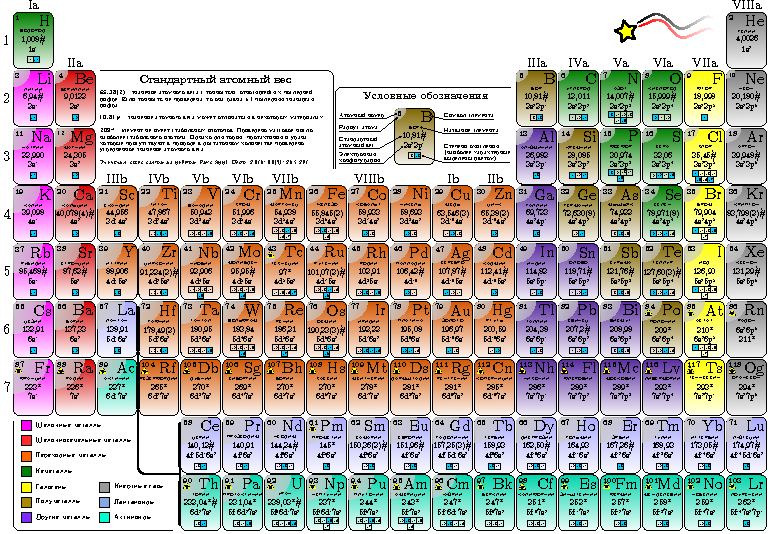
\includegraphics[width=0.9\linewidth, keepaspectratio]{tables/periodic_table.pdf}
    \end{figure}
\end{landscape}

\newpage

\begin{landscape}
    \section{Электроотрицательности химических элементов}\label{appendix:electronegativity}
    \begin{figure}[H]
        \vspace*{-0.5cm}
        \centering
        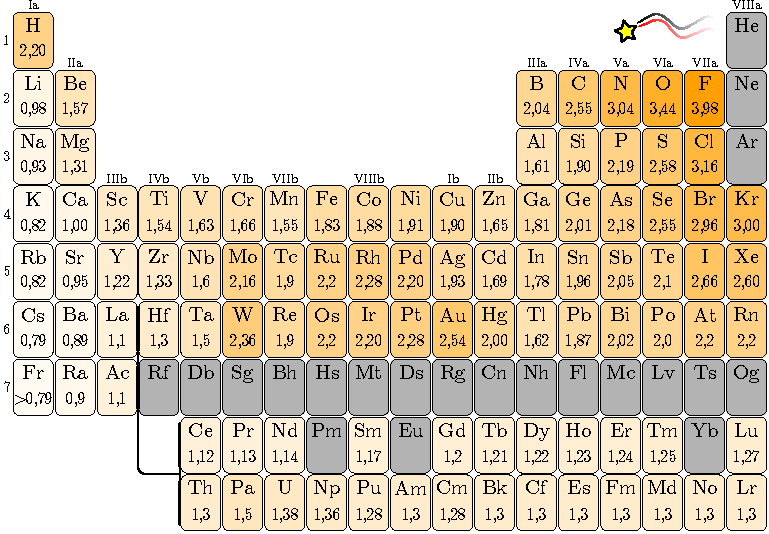
\includegraphics[width=0.9\linewidth, keepaspectratio]{tables/electronegativity.pdf}
    \end{figure}
\end{landscape}

\section{Таблица растворимости солей}\label{appendix:table_of_solubility_of_salts}

\begin{figure}[H]
    \vspace*{-0.5cm}
    \centering
    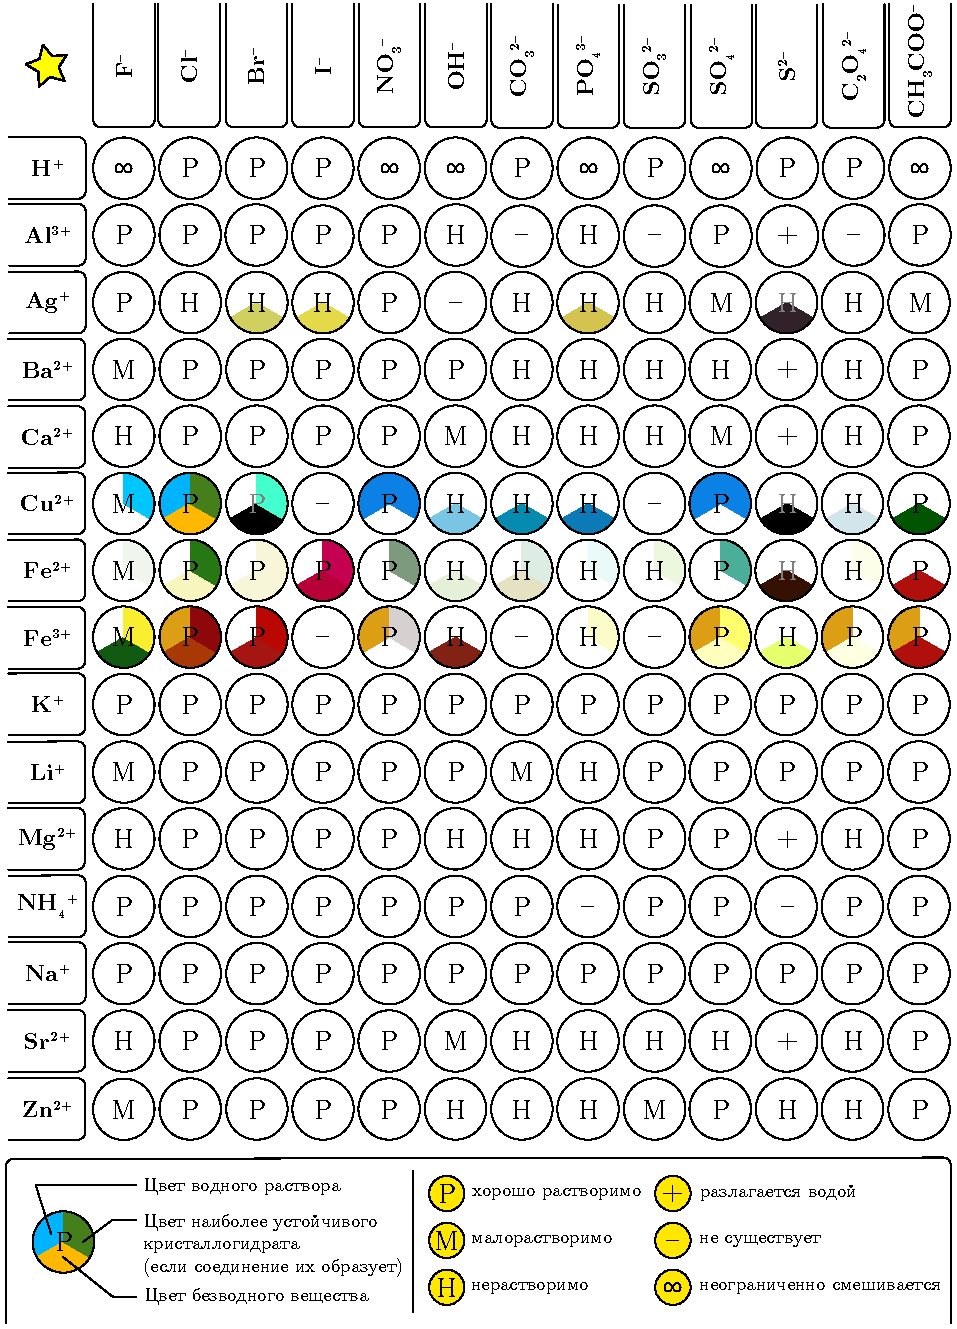
\includegraphics[width=14.5cm]{tables/table_of_solubility_part_1.pdf}
\end{figure}

\newpage

\textbf{Таблица растворимости солей (продолжение)}

\begin{figure}[htbp]
    \centering
    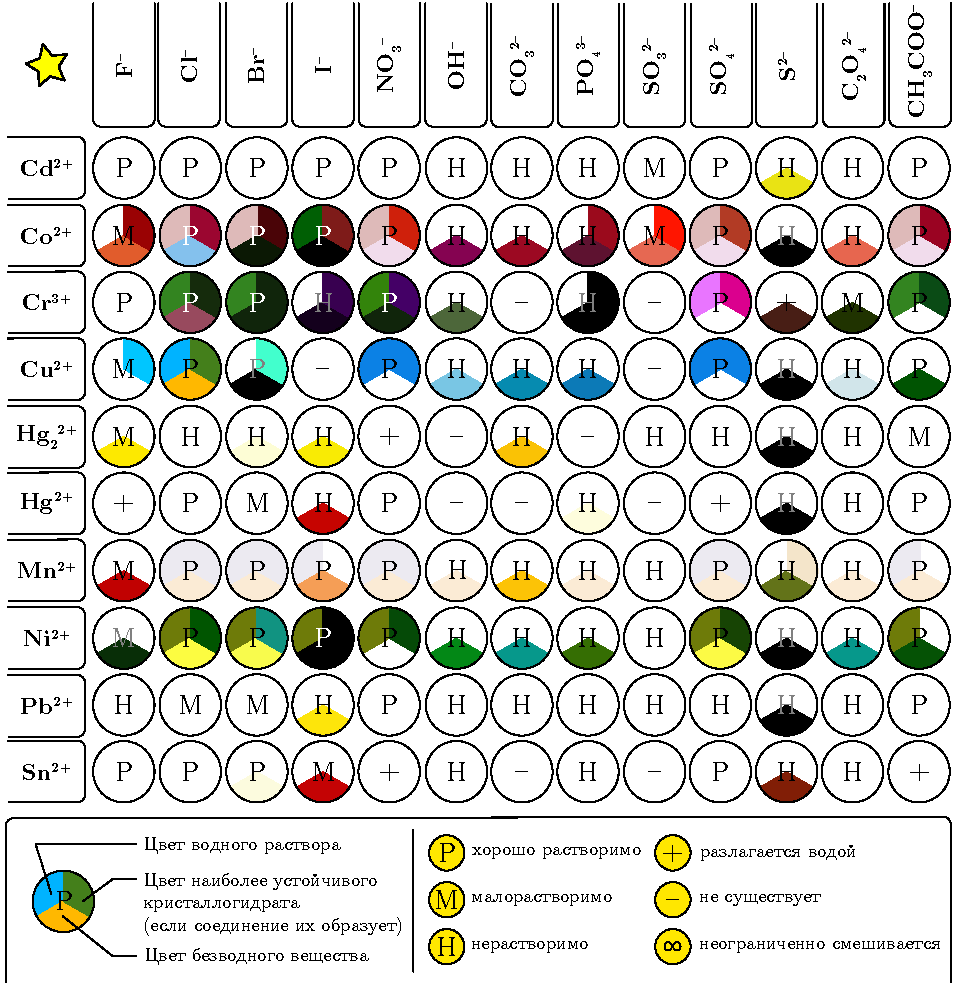
\includegraphics[width=14.5cm]{tables/table_of_solubility_part_2.pdf}
\end{figure}

\restoregeometry
\titlespacing{\section}{0pt}{*6}{*6}
\pagestyle{plain}

\newpage

\renewcommand{\thesection}{\Alph{section}}
\pagestyle{empty}
\titlespacing{\section}{0pt}{*4}{*2}

\section{Степени окисления химических элементов}\label{appendix:oxidation_states_of_chemical_elements}

Жёлтым цветом обозначены наиболее устойчивые степени окисления.

\begin{table}[H]
    \small
    \begin{tabularx}{\textwidth}{
        >{\hsize=1\hsize}Z
        >{\hsize=1\hsize}Z
        >{\hsize=1\hsize}Z
        >{\hsize=1\hsize}Z
        >{\columncolor{green!25}\hsize=1\hsize}Z
        >{\hsize=1\hsize}Z
        >{\hsize=1\hsize}Z
        >{\hsize=1\hsize}Z
        >{\hsize=1\hsize}Z
        >{\hsize=1\hsize}Z
        >{\hsize=1\hsize}Z
        >{\hsize=1\hsize}Z
        >{\hsize=1\hsize}Z
        }
        \hline
        &  &  & \cellcolor{yellow!40}-1 & H & \cellcolor{yellow!40}+1 &  &  &  &  &  &  & \\
        &  &  &  & He &  &  &  &  &  &  &  & \\
        &  &  &  & Li & \cellcolor{yellow!40}+1 &  &  &  &  &  &  & \\
        &  &  &  & Be &  & \cellcolor{yellow!40}+2  &  &  &  &  &  & \\
        &  &  &  & B &  &  & \cellcolor{yellow!40}+3 &  &  &  &  & \\
        \cellcolor{yellow!40}-4 & -3 & -2 & -1 & C & +1 & \cellcolor{yellow!40}+2 & +3 & \cellcolor{yellow!40}+4 &  &  &  & \\
        & \cellcolor{yellow!40}-3 & -2 & -1 & N & +1 & +2 & \cellcolor{yellow!40}+3 & +4 & \cellcolor{yellow!40}+5 &  &  & \\
        &  & \cellcolor{yellow!40}-2 & -1 & O & +1 & +2 &  &  &  &  &  & \\
        &  &  & \cellcolor{yellow!40}-1 & F &  &  &  &  &  &  &  & \\
        &  &  &  & Ne &  &  &  &  &  &  &  & \\
        &  &  & -1 & Na & \cellcolor{yellow!40}+1 &  &  &  &  &  &  & \\
        &  &  &  & Mg &  & \cellcolor{yellow!40}+2 &  &  &  &  &  & \\
        &  &  &  & Al & +1 &  & \cellcolor{yellow!40}+3 &  &  &  &  & \\
        \cellcolor{yellow!40}-4 & -3 & -2 & -1 & Si & +1 & +2 & +3 & \cellcolor{yellow!40}+4 &  &  &  & \\
        & \cellcolor{yellow!40}-3 & -2 & -1 & P & +1 & +2 & \cellcolor{yellow!40}+3 & +4 & \cellcolor{yellow!40}+5 &  &  & \\
        &  & \cellcolor{yellow!40}-2 & -1 & S & +1 & +2 & +3 & \cellcolor{yellow!40}+4 & +5 & \cellcolor{yellow!40}+6 &  & \\
        &  &  & \cellcolor{yellow!40}-1 & Cl & \cellcolor{yellow!40}+1 & +2 & \cellcolor{yellow!40}+3 & +4 & \cellcolor{yellow!40}+5 & +6 & \cellcolor{yellow!40}+7 & \\
        &  &  &  & Ar &  &  &  &  &  &  &  & \\
        &  &  &  & K & \cellcolor{yellow!40}+1 &  &  &  &  &  &  & \\
        &  &  &  & Ca &  & \cellcolor{yellow!40}+2 &  &  &  &  &  & \\
        &  &  &  & Sc & +1 & +2 & \cellcolor{yellow!40}+3 &  &  &  &  & \\
        &  &  &  & Ti &  & +2 & +3 & \cellcolor{yellow!40}+4 &  &  &  & \\
        &  &  &  & V & +1 & +2 & +3 & +4 & \cellcolor{yellow!40}+5 &  &  & \\
        &  & -2 & -1 & Cr & +1 & +2 & \cellcolor{yellow!40}+3 & +4 & +5 & \cellcolor{yellow!40}+6 &  & \\
        & -3 & -2 & -1 & Mn & +1 & \cellcolor{yellow!40}+2 & +3 & \cellcolor{yellow!40}+4 & +5 & +6 & \cellcolor{yellow!40}+7 & \\
        &  & -2 & -1 & Fe & +1 & \cellcolor{yellow!40}+2 & \cellcolor{yellow!40}+3 & +4 & +5 & +6 &  & \\
        &  &  & -1 & Co & +1 & \cellcolor{yellow!40}+2 & \cellcolor{yellow!40}+3 & +4 & +5 &  &  & \\
        &  &  & -1 & Ni & +1 & \cellcolor{yellow!40}+2 & +3 & +4 &  &  &  & \\
        \hline
    \end{tabularx}
\end{table}

\newpage

\begin{table}[H]
    \small
    \begin{tabularx}{\textwidth}{
        >{\hsize=1\hsize}Z
        >{\hsize=1\hsize}Z
        >{\hsize=1\hsize}Z
        >{\hsize=1\hsize}Z
        >{\columncolor{green!25}\hsize=1\hsize}Z
        >{\hsize=1\hsize}Z
        >{\hsize=1\hsize}Z
        >{\hsize=1\hsize}Z
        >{\hsize=1\hsize}Z
        >{\hsize=1\hsize}Z
        >{\hsize=1\hsize}Z
        >{\hsize=1\hsize}Z
        >{\hsize=1\hsize}Z
        }
        \hline
        &  &  &  & Cu & +1 & \cellcolor{yellow!40}+2 &  &  &  &  &  &  \\
        &  &  &  & Zn &  & \cellcolor{yellow!40}+2 &  &  &  &  &  &  \\
        &  &  &  & Ga &  &  & \cellcolor{yellow!40}+3 &  &  &  &  &  \\
        -4 &  &  &  & Ge &  & +2 &  & \cellcolor{yellow!40}+4 &  &  &  &  \\
        & \cellcolor{yellow!40}-3 &  &  & As &  &  & \cellcolor{yellow!40}+3 &  & \cellcolor{yellow!40}+5 &  &  &  \\
        &  & \cellcolor{yellow!40}-2 &  & Se &  & +2 &  & \cellcolor{yellow!40}+4 &  & \cellcolor{yellow!40}+6 &  &  \\
        &  &  & \cellcolor{yellow!40}-1 & Br & \cellcolor{yellow!40}+1 &  & \cellcolor{yellow!40}+3 &  & \cellcolor{yellow!40}+5 &  &  &  \\
        &  &  &  & Kr &  & +2 &  &  &  &  &  &  \\
        &  &  &  & Rb & \cellcolor{yellow!40}+1 &  &  &  &  &  &  &  \\
        &  &  &  & Sr &  & \cellcolor{yellow!40}+2 &  &  &  &  &  &  \\
        &  &  &  & Y &  &  & \cellcolor{yellow!40}+3 &  &  &  &  &  \\
        &  &  &  & Zr &  &  &  & \cellcolor{yellow!40}+4 &  &  &  &  \\
        &  &  &  & Nb &  &  &  &  & \cellcolor{yellow!40}+5 &  &  &  \\
        &  &  &  & Mo &  &  &  &  &  & \cellcolor{yellow!40}+6 &  &  \\
        &  &  &  & Tc &  &  &  & \cellcolor{yellow!40}+4 &  &  & \cellcolor{yellow!40}+7 &  \\
        &  &  &  & Ru &  &  & +3 & \cellcolor{yellow!40}+4 &  &  &  & \cellcolor{yellow!40}+8 \\
        &  &  &  & Rh &  &  & \cellcolor{yellow!40}+3 &  &  &  &  &  \\
        &  &  &  & Pd &  & \cellcolor{yellow!40}+2 &  & +4 &  &  &  &  \\
        &  &  &  & Ag & \cellcolor{yellow!40}+1 &  &  &  &  &  &  &  \\
        &  &  &  & Cd &  & \cellcolor{yellow!40}+2 &  &  &  &  &  &  \\
        &  &  &  & In &  &  & \cellcolor{yellow!40}+3 &  &  &  &  &  \\
        -4 &  &  &  & Sn &  & \cellcolor{yellow!40}+2 &  & \cellcolor{yellow!40}+4 &  &  &  &  \\
        & -3 &  &  & Sb &  &  & \cellcolor{yellow!40}+3 &  & \cellcolor{yellow!40}+5 &  &  &  \\
        &  & -2 &  & Te &  &  &  & \cellcolor{yellow!40}+4 &  & \cellcolor{yellow!40}+6 &  &  \\
        &  &  & \cellcolor{yellow!40}-1 & I & +1 &  &  &  & \cellcolor{yellow!40}+5 &  & +7 &  \\
        &  &  &  & Xe &  & +2 &  & +4 &  & +6 &  & +8 \\
        &  &  &  & Cs & \cellcolor{yellow!40}+1 &  &  &  &  &  &  &  \\
        &  &  &  & Ba &  & \cellcolor{yellow!40}+2 &  &  &  &  &  &  \\
        &  &  &  & La &  &  & \cellcolor{yellow!40}+3 &  &  &  &  &  \\
        &  &  &  & Ce &  &  & \cellcolor{yellow!40}+3 & +4 &  &  &  &  \\
        \hline
    \end{tabularx}
\end{table}

\newpage

\begin{table}[H]
    \small
    \begin{tabularx}{\textwidth}{
        >{\hsize=1\hsize}Z
        >{\hsize=1\hsize}Z
        >{\hsize=1\hsize}Z
        >{\hsize=1\hsize}Z
        >{\columncolor{green!25}\hsize=1\hsize}Z
        >{\hsize=1\hsize}Z
        >{\hsize=1\hsize}Z
        >{\hsize=1\hsize}Z
        >{\hsize=1\hsize}Z
        >{\hsize=1\hsize}Z
        >{\hsize=1\hsize}Z
        >{\hsize=1\hsize}Z
        >{\hsize=1\hsize}Z
        }
        \hline
        &  &  &  & Pr &  &  & \cellcolor{yellow!40}+3 & +4 &  &  &  &  \\
        &  &  &  & Nd &  &  & \cellcolor{yellow!40}+3 &  &  &  &  &  \\
        &  &  &  & Pm &  &  & \cellcolor{yellow!40}+3 &  &  &  &  &  \\
        &  &  &  & Sm &  &  & \cellcolor{yellow!40}+3 &  &  &  &  &  \\
        &  &  &  & Eu &  & +2 & \cellcolor{yellow!40}+3 &  &  &  &  &  \\
        &  &  &  & Gd &  &  & \cellcolor{yellow!40}+3 &  &  &  &  &  \\
        &  &  &  & Tb &  &  & \cellcolor{yellow!40}+3 & +4 &  &  &  &  \\
        &  &  &  & Dy &  &  & \cellcolor{yellow!40}+3 &  &  &  &  &  \\
        &  &  &  & Ho &  &  & \cellcolor{yellow!40}+3 &  &  &  &  &  \\
        &  &  &  & Er &  &  & \cellcolor{yellow!40}+3 &  &  &  &  &  \\
        &  &  &  & Tm &  &  & \cellcolor{yellow!40}+3 &  &  &  &  &  \\
        &  &  &  & Yb &  & +2 & \cellcolor{yellow!40}+3 &  &  &  &  &  \\
        &  &  &  & Lu &  &  & \cellcolor{yellow!40}+3 &  &  &  &  &  \\
        &  &  &  & Hf &  &  &  & \cellcolor{yellow!40}+4 &  &  &  &  \\
        &  &  &  & Ta &  &  &  &  & \cellcolor{yellow!40}+5 &  &  &  \\
        &  &  &  & W &  &  &  &  &  & \cellcolor{yellow!40}+6 &  &  \\
        &  &  &  & Re &  &  &  & \cellcolor{yellow!40}+4 &  &  & \cellcolor{yellow!40}+7 &  \\
        &  &  &  & Os &  &  &  & \cellcolor{yellow!40}+4 &  &  &  & \cellcolor{yellow!40}+8 \\
        &  &  &  & Ir* &  &  & \cellcolor{yellow!40}+3 & +4 &  &  &  &  \\
        &  &  &  & Pt &  & \cellcolor{yellow!40}+2 &  & \cellcolor{yellow!40}+4 &  & +6 &  &  \\
        &  &  &  & Au & +1 &  & \cellcolor{yellow!40}+3 &  &  &  &  &  \\
        &  &  &  & Hg & +1 & \cellcolor{yellow!40}+2 &  &  &  &  &  &  \\
        &  &  &  & Tl & \cellcolor{yellow!40}+1 &  & \cellcolor{yellow!40}+3 &  &  &  &  &  \\
        &  &  &  & Pb &  & \cellcolor{yellow!40}+2 &  & +4 &  &  &  &  \\
        &  &  &  & Bi &  &  & \cellcolor{yellow!40}+3 &  & +5 &  &  &  \\
        &  &  &  & Po &  & +2 &  & +4 &  &  &  &  \\
        &  &  & -1 & At & +1 &  & +3 &  & +5 &  & +7 &  \\
        &  &  &  & Rn &  & +2 &  &  &  &  &  &  \\
        &  &  &  & Fr & \cellcolor{yellow!40}+1 &  &  &  &  &  &  &  \\
        &  &  &  & Ra &  & \cellcolor{yellow!40}+2 &  &  &  &  &  &  \\
        \hline
    \end{tabularx}
\end{table}

\newpage

\begin{table}[H]
    \small
    \begin{tabularx}{\textwidth}{
        >{\hsize=1\hsize}Z
        >{\hsize=1\hsize}Z
        >{\hsize=1\hsize}Z
        >{\hsize=1\hsize}Z
        >{\columncolor{green!25}\hsize=1\hsize}Z
        >{\hsize=1\hsize}Z
        >{\hsize=1\hsize}Z
        >{\hsize=1\hsize}Z
        >{\hsize=1\hsize}Z
        >{\hsize=1\hsize}Z
        >{\hsize=1\hsize}Z
        >{\hsize=1\hsize}Z
        >{\hsize=1\hsize}Z
        }
        \hline
        &  &  &  & Ac &  &  & \cellcolor{yellow!40}+3 &  &  &  &  &  \\
        &  &  &  & Th &  &  &  & \cellcolor{yellow!40}+4 &  &  &  &  \\
        &  &  &  & Pa &  &  &  &  & \cellcolor{yellow!40}+5 &  &  &  \\
        &  &  &  & U &  &  &  & +4 &  & \cellcolor{yellow!40}+6 &  &  \\
        &  &  &  & Np &  &  &  &  & \cellcolor{yellow!40}+5 &  &  &  \\
        &  &  &  & Pu &  &  &  & \cellcolor{yellow!40}+4 &  &  &  &  \\
        &  &  &  & Am &  &  & \cellcolor{yellow!40}+3 &  &  &  &  &  \\
        &  &  &  & Cm &  &  & \cellcolor{yellow!40}+3 &  &  &  &  &  \\
        &  &  &  & Bk &  &  & \cellcolor{yellow!40}+3 &  &  &  &  &  \\
        &  &  &  & Cf &  &  & \cellcolor{yellow!40}+3 &  &  &  &  &  \\
        &  &  &  & Es &  &  & \cellcolor{yellow!40}+3 &  &  &  &  &  \\
        &  &  &  & Fm &  &  & \cellcolor{yellow!40}+3 &  &  &  &  &  \\
        &  &  &  & Md &  &  & \cellcolor{yellow!40}+3 &  &  &  &  &  \\
        &  &  &  & No &  & +2 &  &  &  &  &  &  \\
        &  &  &  & Lr &  &  & \cellcolor{yellow!40}+3 &  &  &  &  &  \\
        &  &  &  & Rf &  &  &  & +4 &  &  &  &  \\
        &  &  &  & Db &  &  &  &  & +5 &  &  &  \\
        &  &  &  & Sg &  &  &  &  &  & +6 &  &  \\
        &  &  &  & Bh &  &  &  &  &  &  & +7 &  \\
        &  &  &  & Hs &  &  &  &  &  &  &  & +8 \\
        \hline
    \end{tabularx}
\end{table}

* Для иридия в 2014 году была экспериментально подтверждена степень окисления +9 в составе газового катиона \ce{[IrO4]^+}.

\newpage

\begin{landscape}
    \section{Взаимодействие химических элементов с азотной кислотой}\label{appendix:reaction_of_chemical_elements_with_nitric_acid}
    \begin{figure}[H]
        \vspace*{-0.5cm}
        \centering
        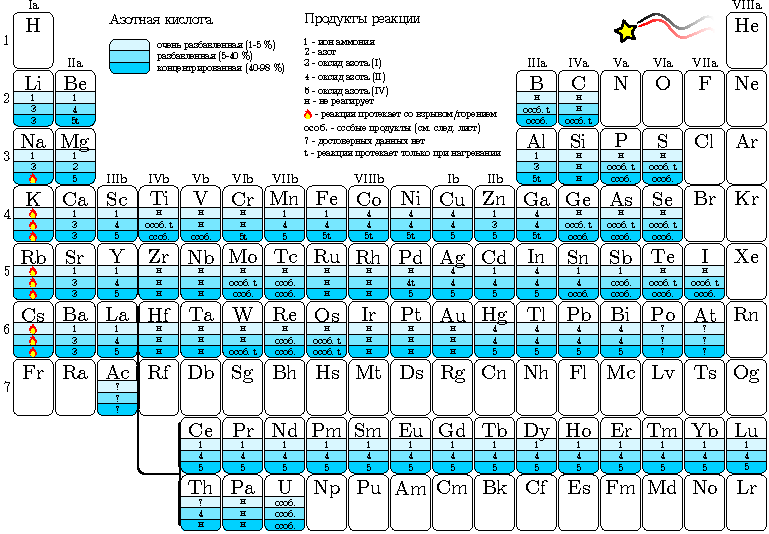
\includegraphics[width=0.9\linewidth, keepaspectratio]{tables/reaction_of_chemical_elements_with_nitric_acid.pdf}
    \end{figure}
\end{landscape}

\newpage

\begin{table}[htbp]
    \small
    \begin{tabularx}{\textwidth}{
        >{\hsize=0.3\hsize}Y
        >{\hsize=1.7\hsize}Y
        }
        \hline
        \rowcolor{green!5}
        Элемент & Уравнение/примечание \\
        \hline
        B & \ce{B + HNO3_{\text{(разб.)}} + H2O ->[\Delta] H3BO3 + NO (^)} \\
        B & \ce{B + 3HNO3_{\text{(конц.)}} -> H3BO3 + 3NO2 (^)} \\
        C & \ce{C + 4HNO3_{\text{(конц.)}} ->[\Delta] CO2 (^) + 4NO2 (^) + 2H2O} \\
        P & \ce{3P + 5HNO3_{\text{(разб.)}} + 2H2O ->[\Delta] 3H3PO4 + 5NO (^)} \\
        P & \ce{P + 5HNO3_{\text{(конц.)}} -> H3PO4 + 5NO2 (^) + H2O} \\
        S & \ce{S + 2HNO3_{\text{(разб.)}} ->[\Delta] H2SO4 + 2NO (^)} \\
        S & \ce{S + 6HNO3_{\text{(конц.)}} -> H2SO4 + 6NO2 (^) + 2H2O } \\
        Ti & \ce{3Ti + 4HNO3_{\text{(разб.)}} + H2O ->[\Delta] 3H2TiO3 (v) + 4NO (^)} \\
        Ti & \ce{Ti + 4HNO3_{\text{(конц.)}} -> H2TiO3 (v) + 4NO2 (^) + H2O} \\
        V & \ce{V + 5HNO3_{\text{(конц.)}} -> HVO3 (v) + 5NO2 (^) + 2H2O} \\
        Ge & \ce{Ge + 4HNO3_{\text{(конц.)}} -> GeO2 (v) + 4NO2 (^) + 2H2O} \\
        As & \ce{As + HNO3_{\text{(разб.)}} + H2O -> H3AsO3 + NO (^)} \\
        As & \ce{As + 5HNO3_{\text{(конц.)}} -> H3AsO4 + 5NO2 (^) + H2O} \\
        Se & \ce{3Se + 4HNO3_{\text{(разб.)}} + H2O ->[\Delta] 3H2SeO3 + 4NO (^)} \\
        Se & \ce{Se + 4HNO3_{\text{(конц.)}} -> H2SeO3 + 4NO2 (^) + H2O} \\
        Mo & \ce{Mo + 6HNO3 -> H2MoO4 (v) + 6NO2 (^) + 2H2O} \\
        Tc & \ce{Tc + 7HNO3 -> HTcO4 + 7NO2 (^) + 3H2O} \\
        Sn & \ce{Sn + 4HNO3_{\text{(конц.)}} -> H2SnO3 (v) + 4NO2 (^) + H2O} \\
        Sb & \ce{2Sb + 2HNO3_{\text{(разб.)}} -> Sb2O3 (v) + 2NO (^) + H2O} \\
        Sb & \ce{Sb + 5HNO3_{\text{(конц.)}} -> HSbO3 (v) + 5NO2 (^) + 2H2O} \\
        Te & \ce{3Te + 4HNO3_{\text{(разб.)}} + H2O ->[\Delta] 3H2TeO3 (v) + 4NO (^)} \\
        Te & \ce{Te + 4HNO3_{\text{(конц.)}} -> H2TeO3 (v) + 4NO2 (^) + H2O} \\
        I & \ce{I2 + 10HNO3_{\text{(конц.)}} ->[\Delta] 2HIO3 + 10NO2 (^) + 4H2O} \\
        W & \ce{W + 6HNO3_{\text{(конц.)}} ->[\Delta] H2WO4 (v) + 6NO2 (^) + 2H2O} \\
        Re & \ce{Re + 7HNO3 -> HReO4 + 7NO2 (^) + 3H2O} \\
        Os & \ce{Os + 8HNO3 ->[\Delta] OsO4 + 8NO2 (^) + 4H2O} \\
        U & \ce{U + 4HNO3_{\text{(разб.)}} -> UO2(NO3)2 + 2NO (^) + 2H2O} \\
        U & \ce{U + 8HNO3_{\text{(конц.)}} -> UO2(NO3)2 + 6NO2 (^) + 4H2O} \\
        \hline
    \end{tabularx}
\end{table}

\newpage

\section{Кислотно-основные индикаторы}\label{appendix:pH_indicator_colors}

\begin{table}[htbp]
    \small
    \begin{tabularx}{\textwidth}{
        >{\hsize=1.6\hsize}Y
        >{\hsize=0.8\hsize}Z
        >{\hsize=0.8\hsize}Z
        >{\hsize=0.8\hsize}Z
        }
        \hline
        \rowcolor{green!5}
        Название индикатора & Цвет в более кислой области & Интервал перехода & Цвет в более щелочной области \\
        \hline
        Метиловый фиолетовый (I) & \cellcolor{methyl_violet_I_acid} & \num{0,0}--\num{1,6} & \cellcolor{methyl_violet_I_base} \\
        \hline
        Метиловый фиолетовый (II) & \cellcolor{methyl_violet_II_acid} & \num{1,6}--\num{2,6} & \cellcolor{methyl_violet_II_base} \\
        \hline
        Тимоловый синий (I) & \cellcolor{thymol_blue_I_acid} & \num{1,2}--\num{2,8} & \cellcolor{thymol_blue_I_base} \\
        \hline
        Метиловый фиолетовый (III) & \cellcolor{methyl_violet_III_acid} & \num{2,6}--\num{3,2} & \cellcolor{methyl_violet_III_base} \\
        \hline
        Метиловый оранжевый & \cellcolor{methyl_orange_acid} & \num{3,1}--\num{4,4} & \cellcolor{methyl_orange_base} \\
        \hline
        Метиловый красный & \cellcolor{methyl_red_acid} & \num{4,4}--\num{6,2} & \cellcolor{methyl_red_base} \\
        \hline
        Лакмус & \cellcolor{litmus_acid} & \num{5,0}--\num{8,0} & \cellcolor{litmus_base} \\
        \hline
        Бромтимоловый синий & \cellcolor{bromthymol_blue_acid} & \num{6,0}--\num{7,6} & \cellcolor{bromthymol_blue_base} \\
        \hline
        Феноловый красный & \cellcolor{phenol_red_acid} & \num{6,8}--\num{8,4} & \cellcolor{phenol_red_base} \\
        \hline
        Тимоловый синий (II) & \cellcolor{thymol_blue_II_acid} & \num{8,0}--\num{9,6} & \cellcolor{thymol_blue_II_base} \\
        \hline
        Фенолфталеин & бесцветный & \num{8,2}--\num{10,0} & \cellcolor{phenolphthalein_base} \\
        \hline
        Индигокармин & \cellcolor{indigo_carmine_acid} & \num{11,6}--\num{14,0} & \cellcolor{indigo_carmine_base} \\
        \hline
    \end{tabularx}
\end{table}

\newpage

\section{Константы кислотности в водных растворах}\label{appendix:acidity_constants_in_aqueous_solutions}

\begin{table}[htbp]
    \small
    \begin{tabularx}{\textwidth}{
        >{\hsize=2.2\hsize}Y
        >{\hsize=0.8\hsize}Y
        >{\hsize=0.5\hsize}Y
        >{\hsize=1\hsize}Y
        >{\hsize=0.5\hsize}Y
        }
        \hline
        \rowcolor{green!5}
        Кислота & Формула & $t$, \unit{\degreeCelsius} & $K_a$ & $\text{p}K_a$ \\
        \hline
        Азотная & \ce{HNO3} & 25 & & $< 0$ \\
        Азотоводородная & \ce{HN3} & 20 & \num{2,09e-5} & \num{4,68} \\
        Борная (мета) & \ce{HBO2} & 18 & \num{7,5e-10} & \num{9,12} \\
        Борная (орто) & \ce{H3BO3} & 25 & \num{5,8e-10} & \num{9,24} \\
        Бромоводородная & \ce{HBr} & 25 & & $< 0$ \\
        Бромноватая & \ce{HBrO3} & 18 & \num{2e-1} & \num{0,7} \\
        Бромноватистая & \ce{HBrO} & 25 & \num{2,06e-9} & \num{8,7} \\
        Дихромовая & \ce{H2Cr2O7} & 25 & \num{2,3e-2} & \num{1,64} \\
        Иодоводородная & \ce{HI} & 25 & $\sim \num{e11}$ & $< 0$ \\
        Иодная (орто) 1-я ст. & \ce{H5IO6} & 25 & \num{3,09e-2} & \num{1,51} \\
        Иодная (орто) 2-я ст. & \ce{H5IO6} & 25 & \num{7,08e-9} & \num{8,15} \\ 
        Иодная (мета) & \ce{HIO4} & 25 & \num{2,3e-2} & \num{1,64} \\
        Иодноватая & \ce{HIO3} & 25 & \num{1,7e-1} & \num{0,77} \\
        Иодноватистая & \ce{HIO} & 25 & \num{2,29e-11} & \num{10,64} \\
        Кремниевая (мета) 1-я ст. & \ce{H2SiO3} & 18 & \num{2,2e-10} & \num{9,66} \\
        Кремниевая (мета) 2-я ст. & \ce{H2SiO3} & 18 & \num{1,6e-12} & \num{11,80} \\
        Марганцовистая & \ce{H2MnO4} & 25 & \num{7,1e-11} & \num{10,15} \\
        Марганцовая & \ce{HMnO4} & 25 & & $< 0$ \\
        Пероксид водорода & \ce{H2O2} & 25 & \num{2,63e-12} & \num{11,58} \\
        Селенистая 1-я ст. & \ce{H2SeO3} & 25 & \num{3,5e-3} & \num{2,26} \\
        Селенистая 2-я ст. & \ce{H2SeO3} & 25 & \num{5e-8} & \num{7,3} \\
        Селеноводородная 1-я ст. & \ce{H2Se} & 18 & \num{1,7e-4} & \num{3,77} \\
        Селеноводородная 2-я ст. & \ce{H2Se} & 18 & \num{e-11} & \num{11,0} \\
        Селеновая 1-я ст. & \ce{H2SeO4} & 25 & & $< 0$ \\
        Селеновая 2-я ст. & \ce{H2SeO4} & 25 & \num{1,2e2} & \num{1,9} \\
        Селеноциановая & \ce{HSeCN} & 25 & \num{2,19e-2} & \num{1,66} \\
        Серная 1-я ст. & \ce{H2SO4} & 25 & & $< 0$ \\
        Серная 2-я ст. & \ce{H2SO4} & 25 & \num{1,2e-2} & \num{1,9} \\
        \hline
    \end{tabularx}
\end{table}

\newpage

\begin{table}[htbp]
    \small
    \begin{tabularx}{\textwidth}{
        >{\hsize=2.2\hsize}Y
        >{\hsize=0.8\hsize}Y
        >{\hsize=0.5\hsize}Y
        >{\hsize=1\hsize}Y
        >{\hsize=0.5\hsize}Y
        }
        \hline
        \rowcolor{green!5}
        Кислота & Формула & $t$, \unit{\degreeCelsius} & $K_a$ & $\text{p}K_a$ \\
        \hline
        Сернистая 1-я ст. & \ce{H2SO3} & 25 & \num{1,58e-2} & \num{1,8} \\
        Сернистая 2-я ст. & \ce{H2SO3} & 25 & \num{6,3e-8} & \num{7,2} \\
        Сероводородная 1-я ст. & \ce{H2S} & 25 & \num{6e-8} & \num{7,2} \\
        Сероводородная 1-я ст. & \ce{H2S} & 25 & \num{e-14} & \num{14,0} \\
        Сульфаминовая & \ce{NH2SO2OH} & 25 & \num{9,77e-2} & \num{1,01} \\
        Телуроводородная & \ce{H2Te} & 25 & \num{e-3} & \num{3,0} \\
        Тетраборная 1-я ст. & \ce{H2B4O7} & 25 & \num{e-4} & \num{4} \\
        Тетраборная 2-я ст. & \ce{H2B4O7} & 25 & \num{e-9} & \num{9} \\
        Тетрафторборная & \ce{H[BF4]} & 25 & & $< 0$ \\
        Тиосерная 1-я ст. & \ce{H2S2O3} & 25 & \num{2,2e-1} & \num{0,66} \\
        Тиосерная 2-я ст. & \ce{H2S2O3} & 25 & \num{2,8e-2} & \num{1,56} \\
        Тиоциановая & \ce{HSCN} & 18 & \num{1,4e-1} & \num{0,85} \\
        Тритиоугольная 1-я ст. & \ce{H2CS3} & 20 & \num{2,09e-3} & \num{2,68} \\
        Тритиоугольная 2-я ст. & \ce{H2CS3} & 20 & \num{6,03e-9} & \num{8,22} \\
        Угольная (истинная) & \ce{H2CO3} & 25 & \num{1,32e-4} & \num{3,88} \\
        Угольная (кажущаяся) 1-я ст.* & \ce{H2CO3} & 25 & \num{4,45e-7} & \num{6,35} \\
        Угольная (кажущаяся) 2-я ст. & \ce{H2CO3} & 25 & \num{4,69e-11} & \num{10,33} \\
        Уксусная & \ce{CH3COOH} & 25 & \num{1,75e-5} & \num{4,76} \\
        Фосфористая 1-я ст. & \ce{H3PO3} & 25 & \num{1,6e-2} & \num{1,80} \\
        Фосфористая 2-я ст. & \ce{H3PO3} & 25 & \num{6,3e-7} & \num{6,2} \\
        Фосфорная (орто) 1-я ст. & \ce{H3PO4} & 25 & \num{7,52e-3} & \num{2,12} \\
        Фосфорная (орто) 2-я ст. & \ce{H3PO4} & 25 & \num{6,31e-8} & \num{7,20} \\
        Фосфорная (орто) 3-я ст. & \ce{H3PO4} & 25 & \num{4,47e-13} & \num{12,35} \\
        Фосфорноватистая & \ce{H2PO2} & 25 & \num{7,9e-2} & \num{1,1} \\
        Фтороводородная & \ce{HF} & 25 & \num{6,61e-4} & \num{3,13} \\
        Фтороводородная (димер) & \ce{H2F2} & 25 & \num{2,63e-3} & \num{2,58} \\
        Фторофосфорная 1-я ст. & \ce{H2[PO3F]} & 25 & \num{2,8e-1} & \num{0,55} \\
        Фторофосфорная 2-я ст. & \ce{H2[PO3F]} & 25 & \num{1,5e-5} & \num{4,80} \\
        \hline
    \end{tabularx}
\end{table}

* Термин <<кажущаяся константа>> означает, что данная константа отнесена к общему количеству \ce{CO2} в растворе.

\newpage

\begin{table}[htbp]
    \small
    \begin{tabularx}{\textwidth}{
        >{\hsize=2.2\hsize}Y
        >{\hsize=0.8\hsize}Y
        >{\hsize=0.5\hsize}Y
        >{\hsize=1\hsize}Y
        >{\hsize=0.5\hsize}Y
        }
        \hline
        \rowcolor{green!5}
        Кислота & Формула & $t$, \unit{\degreeCelsius} & $K_a$ & $\text{p}K_a$ \\
        \hline
        Хлористая & \ce{HClO2} & 18 & \num{5e-3} & \num{2,3} \\
        Хлороводородная (соляная) & \ce{HCl} & 25 & & $< 0$ \\
        Хлорная & \ce{HClO4} & 25 & & $< 0$ \\
        Хлорноватистая & \ce{HClO} & 25 & \num{5,01e-8} & \num{7,3} \\
        Хлорсульфоновая & \ce{ClSO3H} & 20 & & $< 0$ \\
        Хромовая 1-я ст. & \ce{H2Cr2O7} & 25 & & $< 0$ \\
        Хромовая 2-я ст. & \ce{H2Cr2O7} & 25 & \num{3,16e-7} & \num{6,50} \\
        Циановодородная (синильная) & \ce{HCN} & 25 & \num{7,9e-10} & \num{9,1} \\
        Циановая & \ce{HCNO} & 18 & \num{1,2e-4} & \num{3,92} \\
        \hline
    \end{tabularx}
\end{table}

\newpage

\section{Константы основности в водных растворах}\label{appendix:basicity_constants_in_aqueous_solutions}

\begin{table}[htbp]
    \small
    \begin{tabularx}{\textwidth}{
        >{\hsize=2.1\hsize}Y
        >{\hsize=1\hsize}Y
        >{\hsize=0.5\hsize}Y
        >{\hsize=0.9\hsize}Y
        >{\hsize=0.5\hsize}Y
        }
        \hline
        \rowcolor{magenta!5}
        Основание & Формула & $t$, \unit{\degreeCelsius} & $K_b$ & $\text{p}K_b$ \\
        \hline
        Алюминия гидроксид & \ce{Al(OH)2} & 25 & \num{1,38e-9} & \num{8,86} \\
        Аммиака гидрат & \ce{NH3*H2O} & 25 & \num{1,79e-5} & \num{4,75} \\
        Бария гидроксид & \ce{Ba(OH)2} & 25 & \num{2,3e-1} & \num{0,64} \\
        Гидразина гидрат & \ce{N2H4*H2O} & 25 & \num{1,2e-6} & \num{5,9} \\
        Гидроксиламина гидрат & \ce{NH2OH*H2O} & 25 & \num{9,33e-9} & \num{8,03} \\
        Железа (II) гидроксид & \ce{Fe(OH)2} & 25 & \num{1,3e-4} & \num{3,89} \\
        Железа (III) гидроксид 1-я ст. & \ce{Fe(OH)3} & 25 & \num{1,82e-11} & \num{10,74} \\
        Железа (III) гидроксид 2-я ст. & \ce{Fe(OH)3} & 25 & \num{1,35e-12} & \num{11,87} \\
        Кадмия (II) гидроксид & \ce{Cd(OH)2} & 30 & \num{5,0e-3} & \num{2,30} \\
        Кальция гидроксид & \ce{Ca(OH)2} & 25 & \num{4,3e-2} & \num{1,37} \\
        Кобальта (II) гидроксид & \ce{Co(OH)2} & 25 & \num{4e-5} & \num{4,4} \\
        Лития гидроксид & \ce{LiOH} & 25 & \num{6,75e-1} & \num{0,17} \\
        Магния гидроксид & \ce{Mg(OH)2} & 25 & \num{2,5e-3} & \num{2,60} \\
        Марганца (II) гидроксид & \ce{Mn(OH)2} & 30 & \num{5,0e-4} & \num{3,30} \\
        Меди (II) гидроксид & \ce{Cu(OH)2} & 25 & \num{3,4e-7} & \num{6,47} \\
        Никеля (II) гидроксид & \ce{Ni(OH)2} & 30 & \num{2,5e-5} & \num{4,60} \\
        Свинца (II) гидроксид & \ce{Pb(OH)2} & 25 & \num{9,6e-4} & \num{3,02} \\
        Серебра (I) гидроксид & \ce{AgOH} & 25 & \num{1,1e-4} & \num{3,96} \\
        Стронция гидроксид & \ce{Sr(OH)2} & 25 & \num{1,50e-1} & \num{0,82} \\
        Хрома (III) гидроксид & \ce{Cr(OH)3} & 25 & \num{1,02e-10} & \num{9,99} \\
        Цинка гидроксид & \ce{Zn(OH)2} & 25 & \num{4e-5} & \num{4,4} \\
        \hline
    \end{tabularx}
\end{table}